\documentclass{article}
\usepackage{amssymb}
\usepackage{tikz}

\begin{document}

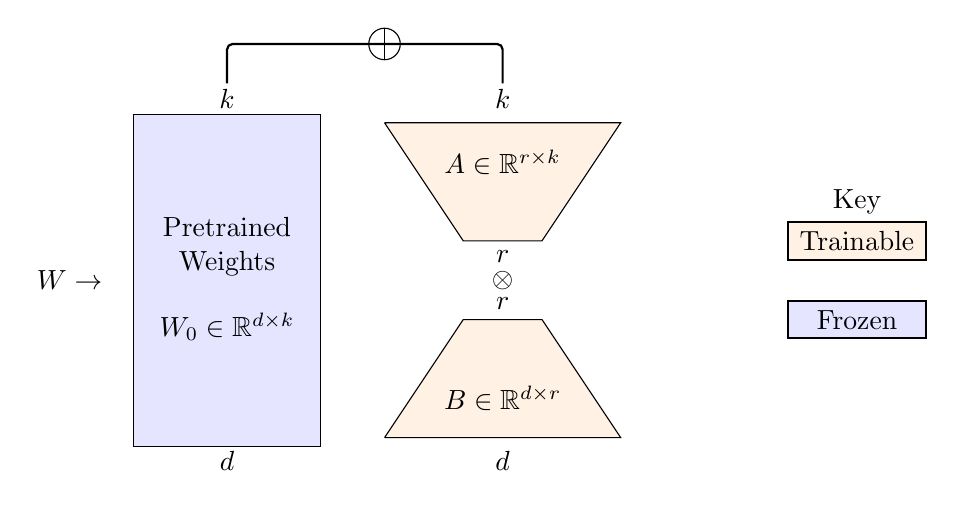
\begin{tikzpicture}[]
\node[fill=blue!10 ,minimum height = 12em, draw=black] at (0,0) {\begin{tabular}{c}Pretrained\\ Weights\\ \\ $W_0 \in \mathbb{R}^{d\times k}$ \end{tabular}};

\draw[fill=orange!10 ,minimum height = 10em] (2,-2) -- (5,-2) -- (4,-.5) -- (3,-.5) -- (2,-2);
\draw[fill=orange!10 ,minimum height = 10em] (2,2) -- (5,2) -- (4,.5) -- (3,.5) -- (2,2);
\node at (3.5,-1.5) {$B\in \mathbb{R}^{d\times r}$};
\node at (3.5,1.5) {$A\in \mathbb{R}^{r\times k}$};
\node at (3.5,0) {$\otimes$};
\node at (3.5,.3) {$r$};
\node at (3.5,-.3) {$r$};
\node at (3.5,-2.3) {$d$};
\node at (0,-2.3) {$d$};
\node at (0,2.3) {$k$};
\node at (3.5,2.3) {$k$};
\draw (2,3) circle (2mm);
\draw (2,3-.2) -- (2,3+.2);
\draw[rounded corners=2pt, thick] (0,2.5) |- (2,3);
\draw[rounded corners=2pt, thick] (3.5,2.5) |- (2,3);
\node[fill=orange!10, draw=black, thick, minimum width=5em] at (8,0.5) {Trainable};
\node[fill=blue!10, draw=black, thick, minimum width=5em] at (8,-0.5) {Frozen};
\node at (8,1) {Key};
\node at (-2,0) {$W \to $};
\end{tikzpicture}

\end{document}